%!TEX root = ../thesis.tex

\cleardoublepage
\chapter{Requirements}
\label{cha:requirements}

%To discuss the solution implemented for this thesis requires a review of, firstly, the requirements contained in the problem statement, and, secondly, a description of both the decisions made as well as the process behind making those decisions. To that extent, this chapter will discuss, the components needed in order to address the problem statement. It will try to discuss not only what decisions were made, but also, crucially, what decisions were \textit{not} made, and why. The first section will begin with the fundamental nature of the solution's architecture, thereafter a review of the design requirements which arise from the Deterministic Networking specification will follow, finally the precise nature of the solution's internal workings will be presented.


To discuss the solution implemented for this thesis requires a review of the requirements contained in the problem statement. Concretely, a multipath backhaul solution, as was described in the introduction, will need to be able to transport the 5G traffic from the edge deployment to the core, while respecting the traffic's QoS requirements. On the condition that this must occur in the presence of more than one backhaul option, this breaks down the problem into a short list of hard requirements.

\begin{enumerate}
  \item Flow Identification


This is a simple requirement but implementing it efficiently can be a challenge \cite{tongaonkar2004fast}. Flow identification is a basic and unavoidable requirement for this system. All IP packets the WAN Connector receives must be identified and mapped to their appropriate Flow Descriptions. A flow description may match one or more flows, but any single flow should only ever map back to one flow description. Though it is possible for a flow to match more than one flow description, in these instances a tiebreaker can be used: either whichever flow description was seen first or whichever has the higher priority. Packets from flows which do not match any description must be dropped. Packets for flows matching a flow description will need the QoS requirements of the flow description to be upheld.


  \item Management of Multiple Outgoing Paths

Both the WAN Connector in the core and the one in the remote 5G Campus must be able to co-ordinate about their available interfaces and/or IP addresses. By doing so they should be able to determine how many paths there are between them. Furthermore it is desirable to perform path management and observe the paths' characteristics. These characteristics are the bandwidth, jitter, latency, packet loss, as well as status (i.e. if the path is completely broken). A path's characteristics are also not guaranteed to be symmetric so path's will have to be managed based on their direction as well. This requires a complex degree of co-ordination between the remote WAN Connector instances. 

  \item Path Selection in Pursuit of Determinism

It is not enough just to map incoming packets to their QoS requirements, these must also be enforced to as high a degree as possible.  Determinism means that a flow can expect it's QoS to be upheld, provided the network is physically able to do so. As long as some path exists which has a latency less than that required by the flow, then the flow's latency requirements should be met. The same applies to packet loss, jitter, and bandwidth. This also means if there are two paths with sufficiently low jitter and delay, and one of them is down, then the flow should be switched to the other path, or it should be replicated across both paths so that one path going down is not even noticeable.

This is the core building block of this work. Although the previous requirements are all unavoidable, they are all in service of this requirement. It should also be clarified at this point that a flow with QoS requirements which the WAN Connector deems unattainable may be rejected. This does not constitute failure, provided the WAN Connector has correctly deduced that the backhaul paths are all truly insufficient in their current state. If the network is physically unable to provide the flow's desired characteristics then the WAN Connector should reject that flow.

\item Packet Tunneling to Remote Destination

With the flow identification, path management, and path selection all in place, the incoming packets must still be tunneled to the terminating WAN Connector, which forwards them on to their destination. This is the final requirement of such a system. After incoming packets are mapped to a flow, and the path on which that flow should be forwarded has been chosen (based on the data collected about those paths), the packets must still be sent across one of the backhaul paths. Crucially, the flow's source and destination should not have to be aware of the WAN Connector, this means packets must arrive unchanged.

\end{enumerate} 

%%=========================================
%%=========================================
%%=========================================
\cleardoublepage
\chapter{Design}
\label{cha:design}

This chapter reviews the ways in which the requirements of the previous chapter can be met. It will discuss the components needed in order to address the problem statement. It will try to discuss not only what decisions were made, but also, crucially, what decisions were \textit{not} made, and why. The first section will begin with the fundamental structure of the solution's architecture, thereafter an overview of the functionality required will be given. The Deterministic Networking specification will heavily inform these choices, and is referenced repeatedly throughout this chapter.


%%=========================================
\section{Skeleton Structure}
\label{sec:approach:plan}

From the outset it was decided to use a control-user plane split. The packet processing and forwarding is performed in the user plane, and the control plane makes the high level decisions about which packets to send where, and in this case, on which outgoing interface to send them. The data plane is simple and only performs the time critical packet processing, and blindly follows the instructions of the control plane. This type of architecture is common in modern software-based networks, for example OpenFlow, the Evolved Packet Core (from LTE), and the 5G core all implement this kind of control-data plane split.

However, this decision immediately locks one into certain positions. For example, this requires a method of communication between the data plane and the control plane, it also means that the state machine that represents the WAN Connector becomes more complex, and complexity always brings with it a greater danger for hidden mistakes and fallacies. The benefit is that the user plane function does not need any complex decision making logic, thus simplifying its internal architecture. Further, these separate components can then be deployed at different locations, and scaled up or out with greater ease.

%%=========================================
\section{Components Required for Deterministic Multipath Backhaul in a 5G Campus Environment}
\label{sec:approach:comp}

Determinism, in a networking context, refers to the ability of a network to supply specific QoS requirements with extremely high degrees of certainty. IP flows and applications running in these networks are assured bounded latency, jitter, and packet loss. To that extent, while the Deterministic Networking (DetNet) specification comes with several recommendations for how to achieve determinism it does not define determinism. A network which does not fully comply to these specifications may still call itself determinstic (but it may not say it is a DetNet). Since this thesis aims to provide determinstic backhaul, it is not required to follow the DetNet specifications in any form. Though, it does make sense to consider what solutions they have proposed for determinism, since ultimately the goals are the same. In this section, therefore, the DetNet specifications will be used as a source of inspiration for ideas, but not as an absolute source of truth.

Deterministic networks have been discussed in the background chapter. In order to guarantee determinism the IETF DetNet working group has proposed an architecture for determinism over IP networks \cite{detnet-arch}. Their specification identifies four key mechanisms for guaranteeing the determinism of a flow: 1) elimination of contention loss, 2) jitter reduction, 3) service protection, and 4) explicit routes. Since the 5G campus environment may need to use the infrastructure of other operators this rules out the ability to use explicit routes. A key difference between deterministic networks and 5G campus backhaul networks is that the operator may not control all the links between nodes, and that there are only two nodes in the network that are definitely under the administrator's control- the WAN Connectors at the core and the edge. In such a scenario the problem is less like a network and more like a client-server application with multiple paths between the client and the server.

\subsection{Elimination of Contention Loss and Bufferbloat}

Contention between flows must be carefully managed in order to prevent packet loss due to buffer overflows, and, just as importantly, to prevent high latencies due to bufferbloat or excessive queuing. A greedy flow, which uses too much bandwidth, or the presence of too many flows, whose cumulative bandwidth demands exceed the link's capabilities, will have negative effects on all the flows running over the link.

Elimination of contention loss can be achieved by using a traffic shaper and/or rate limiter, and the ingress to any DetNet domain \textbf{must} apply such a function. Therefore a traffic shaper should be applied to the ingress traffic entering the WAN Connector from the RAN, before it is sent across the backhaul links. Since the implementation of a traffic shaper is beyond the scope of this thesis, an existing solution must be used. The traffic control subsystem in the linux kernel (tc) provides several implementations of different algorithms for both rate limiting and traffic shaping. For the purposes of this solution several algorithms were considered: Hierarchical Token Bucket (HTB), Hierarchical Fair Service Curve (HFSC) \cite{stoica1997hierarchical}, Time Aware Priority Queuing (taprio), Common Applications Kept Enhanced (CAKE) \cite{hoiland2018piece}, and Fair Queuing with Controlled Delay (FQ\_CoDel).

For HTB and HFSC, due to the implementation of these algorithms in the linux tc subsystem, integrating them within the context of this solution would require filters for each flow. This is not yet necessarily a hindrance, however it would introduce additional overhead upon the creation and/or addition of each new flow. Perhaps more importantly, the implementation of the HTB algorithm provides no means for fair queuing. This means that while it is not possible for greedy and/or malicious flows to use up the bandwidth of other flows because HTB guarantees bandwidth, the greedy flows can cause other flows to experience higher latency because it does not guarantee delay. The HFSC algorithm improves on this by offering both bandwidth and delay guarantees. However this makes it far more difficult to configure, and would require precise calculation of the service curve for each new flow.

Another feasible option available in linux tc would be time aware priority queuing (taprio). This queuing discipline provides scheduled gates for specific traffic classes. It could be used to schedule flows according to their requirements and/or priorities, and thus provide a form of prioritization, and, to an extent, traffic shaping. Flows can be assigned different windows, and congestion due to a greedy flow is avoided if the greedy flow is scheduled for a different window. However one issue is that taprio fails to provide fair queuing. Thus it would need to be configured, and possibly adapted, as new flows are added and removed, depending on their priority. Flows of the same priority would have to compete with each other to use the bandwidth available in their assigned window.

Lastly there are FQ\_CoDel and CAKE. Both provide fair queuing as well as active queue management, which means flows are less likely to experience loss due to congestion, particularly congestion caused by one particularly greedy flow. Since the CAKE algorithm was originally designed for routers in home networks, and because WLAN networks are loosely analogous to a 5G campus network (consider the UE's as the Stations, and the Base Station as the Access Point), it makes it an attractive choice. CAKE also allows the use of 8 different priority tins, which fits well with the nature of 5G traffic, where different flows have different priorities.

Finally, on a practical level, the implementation of CAKE in the linux kernel uses the kernel's “skb\_flow\_dissector", which exposes a hook point for eBPF programs \footnote{https://www.kernel.org/doc/html/v5.1/networking/bpf\_flow\_dissector.html\#overview}. Specifically within a 5G context, one could attach an eBPF program that allows CAKE to peek inside of GTP tunnels, and differentiate the flows within them. For all the other algorithms mentioned so far, all of the GTP packets would appear to belong to the same IP flow, and thus none of these algorithms would work at all if the traffic is arriving in a GTP tunnel. This is ultimately the strongest case that can be made for any of the options listed so far. TC does have one other algorithm which hooks into the “skb\_flow\_dissector", namely the Choose and Keep Scheduler (CHOKe) \cite{pan2000choke}, which does perform active queue management, however does not provide fair queuing. This means that while it manages buffers in order to prevent greedy flows from filling them up, it does not guarantee different flows a fair share of the bandwidth, which can still lead to flows experiencing increased delay due to other greedy flows. Appendix \ref{appendix:patch} includes a patch which can be used to create an eBPF program which hooks into the “skb\_flow\_dissector" and removes GPT headers. By loading this eBPF program, the CAKE traffic shaper will also be able to function on packets obscured by GTP.

\subsection{Jitter Reduction and Latency Guarantees}

In the DetNet Architecture specification it is recommended to adopt time synchronization as well as sending “Time of Execution" fields in the application packets, in order to achieve jitter reduction. For this approach, the Precision Time Protocol (PTP) protocol should serve to synchronize time between the two WAN Connectors. Especially since there is an existing implementation- the linuxptp project \footnote{https://linuxptp.sourceforge.net/} -  which extends PTP to work over IP networks. As for the time of execution fields, it is possible to place these in a GTP header, or to combine them with timestamping.

Methods to guarantee latency bounds are not mentioned within the specification but they are important for the multi-path setting. Specifically when backhaul options may include satellite links it becomes important to consider latencies. Additionally, in a multi-path environment, latency can be a useful criteria for selecting between links, and guaranteeing delay becomes easier to do when it is possible to switch away from a link that starts to exhibit increased latency.

\subsection{Service Protection}

In order to protect against equipment failure, it may be recommendable to perform packet replication and/or encoding. To address this, the DetNet specification speaks of both duplication of flows, and coding schemes (e.g. Network Coding \cite{ahlswede2000network}, or Forward Error Correction (FEC)). Network Coding could have been a clever solution, however it would require controlling, or at the very least coordinating, all the nodes in the backhaul network (like other parts of the Deterministic Networking specifications), which makes it infeasible for this situation. However, to guard against equipment failure and/or packet loss, duplication does provide an option.

Another option would be FEC. The first problem, though, is that most FEC schemes work on a continuous stream of bytes, providing correction for bit errors, as opposed to correcting the loss of entire packets. Of course packet loss can be viewed as a large continuous sequence of bit errors, but this still places strenuous demands on the encoding scheme. There are schemes which address this issue; fountain codes, such as Raptor \cite{luby2007raptor} encode the data as multiple discrete symbols. These symbols can be mapped directly to packets, thus protecting against packet loss as opposed to just bit errors.

Unfortunately the open source ecosystem surrounding fountain codes is not as developed as that around other FEC schemes, and, because of the complexity involved in implementing them efficiently, there are few freely available projects or libraries which can be used to encode packets using such a scheme. For reference, \footnote{https://aff3ct.github.io/fec\_libraries.html} maintains a list of C/C++ FEC libraries and projects, and none of them support the Raptor family of fountain codes (all other fountain codes incur high overhead).

Even if it were more feasible to integrate FEC into the backhaul solution it bears questioning how much benefit this would bring. FEC is very powerful in situations with consistently lossy links, however paths over the internet tend to experience loss in bursts, not at a consistent rate. To this extent, it may make more sense to duplicate those flows which require a high degree of reliability. This avoids the overhead of forward error encoding, and the duplication ensures that when there are bursts of packet loss they are smoothed over.

If one does choose to duplicate packets in order to achieve service protection, that means an elimination function is also required, as well as a packet ordering function. This is because multiple packets may arrive on one link before they arrive on the other one. If a packet got lost on the faster path, it may still show up on the slower one and thus the packet forwarding needs to pause until the missing packet arrives. The DetNet specifications provide both a basic and an advanced Packet Ordering Function (POF) algorithm \cite{ietf-detnet-pof-08}. This algorithm can be easily adjusted to also perform the elimination of duplicate packets. The DetNet specification also clarifies how long one should wait to see if a missing packet arrives. This value “cannot be smaller than the delay difference of the paths used by the flow" and is called the $POFMaxDelay$.

\begin{algorithm}[H]
\label{pof-alg}

\tcc{initialization}
\lForEach {flow $f$}{$POFLastSent_f \leftarrow 0$}
\tcc{Start POF logic}
\While{true}{
receive packet $p$, with sequence number $seq\_num$ for $flow  f$\;

\eIf{$seq\_num <= POFLastSent_f + 1$}{
\tcc{eliminate duplicates}
\If{$seq\_num == POFLastSent_f +1$}{
forward $p$\;
$POFLastSent_f = seq\_num$\;
}
}{
\tcc{in a separate thread}
buffer $p$ until $seq\_num = POFLastSent_f + 1$ \textbf{or} $POFMaxDelay_f$ elapses\;
forward $p$\;
$POFLastSent_f = seq\_num$\;
}
}

\caption{Basic POF Algorithm Adjusted for De-Duplication}
\end{algorithm}

The algorithm shown in \ref{pof-alg} is the Basic POF algorithm, with a single addition in line 5. The addition was made to make sure that an incoming packet's sequence number is not lower than the next one we were expecting, in order to properly eliminate duplicates. The algorithm's \textbf{if/else} logic in this representation could be unified in a cleaner way, but it was done this way specifically because it thus requires just one extra \textit{if} condition (in line 5) to be added to the DetNet specification's POF algorithm, and that one change suffices to make it a Packet Ordering \textit{and Elimination} Function (POEF).

\subsection{Multipath Considerations}

While the previous subsections have all considered requirements for determinism in an IP network, the issue of multipathing still remains. For a component which is backhauling over multiple links in an IP networks this means link and/or path selection is required. Traditionally, routers select links primarily based on their ability to route the packet to the destination, and secondarily based on various metrics, which can be defined by the administrator. Routing considerations are not made for the WAN Connector's scenario- it's purpose is to backhaul the traffic from the remote Campus Network deployment to the Core, where the network's own internet gateway can then perform the routing.

At this point it is crucial to differentiate, again, between multihoming and multipathing. Multihomed hosts are able to select one of many links for their outgoing traffic's destination. In multipathing the same link may lead to multiple paths to \textit{different} destinations. When two multihomed hosts communicate with each other multiple different paths are opened up. Multipathing over the internet requires complex data collection about all the links in between the source and the destination, see \cite{ganichev2010yamr, apostolaki2021performance,} for examples of such implementations. This is because multipathing over the internet needs to choose paths with maximally edge-disjoint paths to achieve the best reliability, as well as maximally vertex-disjoint paths in order to reduce the load across all nodes on the path.

The goal of this thesis is to use the link and/or path selection to provide determinism for the flows being backhauled. To this extent, the link selection algorithm must attempt to choose paths which can provide lower latency and jitter than the maximum allowed values of a given flow, as well as meeting the flow's minimum reliability requirements. Another consideration for multipath backhaul environments is that it is also possible to duplicate flows across two links (unlike in traditional backhaul scenarios). It is worth noting that while duplication cannot reduce latency it can improve reliability, since a flow which is duplicated across two paths is far less likely to experience packet loss.

\subsection{Summary of Necessary Features}


Looking back on the previous subsections, the following points (in no particular priority) are identified as mandatory for a deterministic backhaul solution: 1) traffic shaping, 2) path selection according to jitter and latency requirements, 3) service protection (i.e. via packet duplication), 4) packet ordering and de-duplication, and 5) time synchronization. Discussion of the ways in which these point are addressed, or how they are implemented, takes place in the following chapter.

\section{Solution Architecture}

\begin{figure}[h]
    \centering
        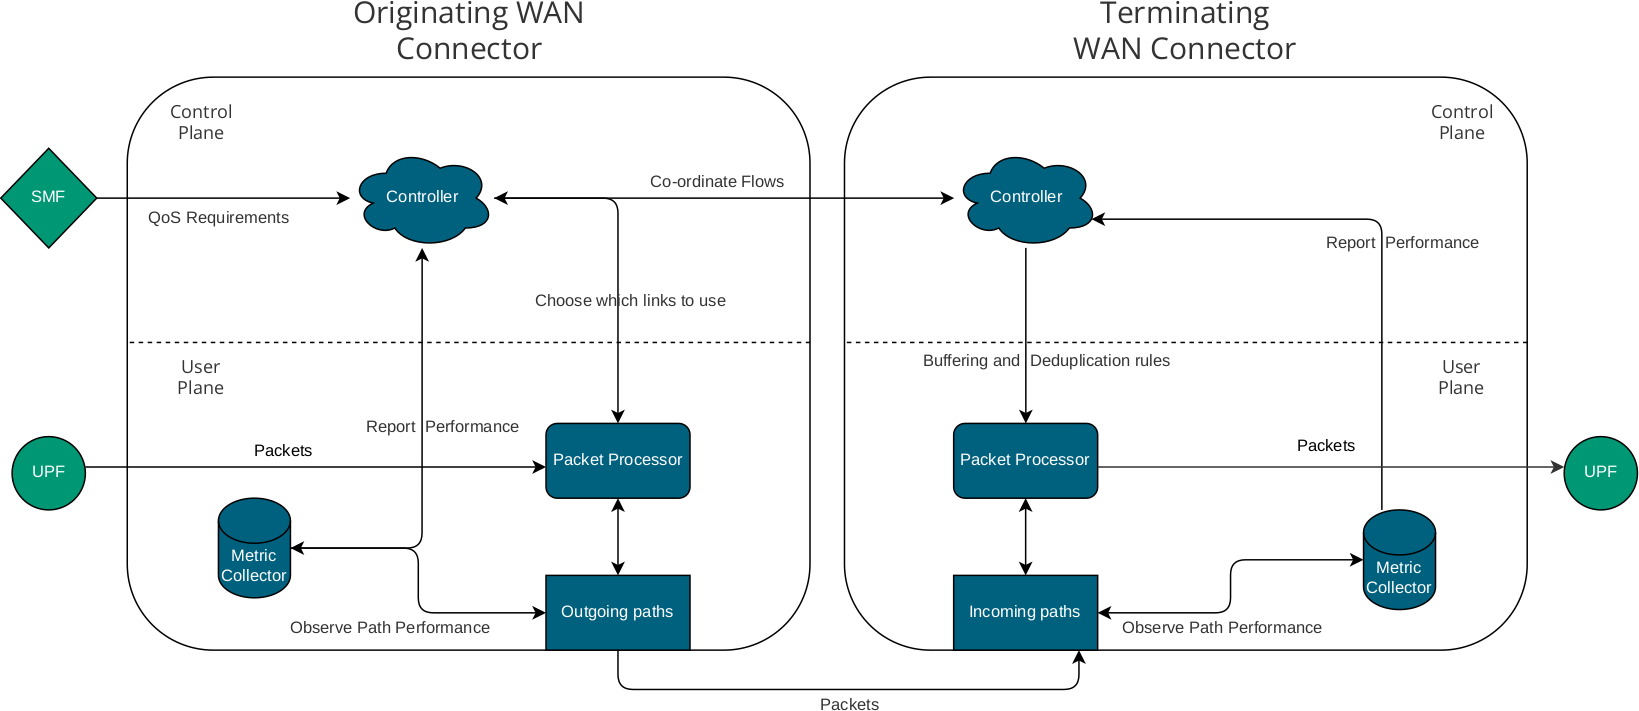
\includegraphics[width=\textwidth]{fig/be-architecture.png}
        \caption{Internal Architecture of the WAN Connector}
        \label{fig:arch}
\end{figure}

Finally, before the next chapter's discussion of the individual components, the design of the internal architecture of the WAN Connector is shown. Figure \ref{fig:arch} illustrates a scenario where the control plane element of the WAN Connector is deployed on the same host that is backhauling traffic to a remote WAN Connector. The diagram is shown for just a single one-way flow. The left side of the diagram is sending the traffic to the right side. Under normal operation there would also be traffic going the other way, and both the “remote" and the “edge" WAN Connector's data planes would be performing the tasks shown in the “sender" and “receiver" boxes. However this representation hopefully makes it easier to understand the tasks that the WAN Connectors will usually perform simultaneously, without cluttering the image. 

The WAN Connector is split into a control plane, which uses the algorithm in \ref{pof-alg} to choose which interfaces to forward on, and a data plane, which performs the forwarding, as well as any necessary buffering, re-ordering and/or de-duplication. Statistics are reported from the user plane back to the control plane. The WAN Connector performs different tasks depending on whether it is the origin or termination of a flow. For example, the terminating node may be receiving duplicate packets on the other paths, and it must know to drop these. Additionally, the sender, can only store statistics about how many bytes it has sent, and on what paths. The receiver, however, is able to use the information contained in the packets it has received to construct a complete picture about the nature of the path - its jitter, latency and also packet loss. The link selector in the control plane can then use this information to make its decisions.

When deploying the WAN Connector there is only one control plane unit (the controller), and two data plane instances. This is because it would be redundant to deploy an additional controller for the remote data plane instance. In the event that each link fails then the remote controller cannot help, even though it can detect it, and if at least one link remains up then the core controller will switch to using that link and can inform the data plane unit to do the same. As has been mentioned before, the graphic depicts a situation in which one of the data plane instances is deployed on the same host as the control plane component. This does not need to be the case, the control plane could also be placed somewhere else entirely, however for the experiments performed in the evaluation chapter, and for the envisioned deployment, this co-location is most likely the easiest to administrate and deploy.

One part which is missing from this diagram is the traffic shaper. That is because it is not connected to the control and the data plane, rather it is meant to be installed alongside them. Furthermore, it is important that the traffic shaper resides in the part of the network before the packets enter the WAN Connector. If the deployment features a UPF in the edge network, it may make sense to place the traffic shaper before this as well. For the core, the traffic shaper will similarly need to be placed at the ingress point where packets first enter the core network.



%%=========================================
%%=========================================
%%=========================================
\cleardoublepage
\chapter{Implementation}
\label{cha:impl}

At this point, one can take the skeleton structure proposed in section \ref{sec:approach:plan} of the previous chapter, and superimpose the other requirements which were determined in section \ref{sec:approach:comp}. Combining these ideas yields the final implementation, which will be now be presented.


%%=========================================

\section{Path Selection Algorithm}

Meeting the various requirements - jitter, latency, and delay - of a flow, via path selection, can be formulated as a multi-constrained QoS problem. Solving such a multi-constrained QoS problem is a binary optimization problem, and the key to deterministically meeting the flow's requirements. The problem can be posed like this: “select those paths on which to forward packets while making sure to satisfy the latency, jitter and reliability requirements of the given flow, and minimizing the overall weight of the paths used". The mathematical definition is as follows:

\begin{gather}
\label{algorithm}
\text{Minimize } \sum_{i=1}^{P}w(x_i) * x_i \\
\text{Where,   } d(i) * x_i\le D \\
j(i) * x_i \le J \\
1 - \prod_{i=1}^{P}{ ( 1- r(i) * x_i ) } \ge R  \\
\text{for } x_i \in \{0,1\}
\end{gather}

Here the variables $D$, $J$, and $R$ are the flow's delay, jitter, and reliability requirements, while the functions $d(i)$, $j(i)$, $r(i)$, $w(i)$ are the estimated delay, jitter, reliability, and weight of link $i$. The predicted values will usually just be the latest measurement, as recommended in \cite{akella2008performance}, however there is room here to define more advanced functions to predict the future link quality and thus perform preemptive path switching. But this is a topic for future work. The total number of paths is $P$. The $x_i$ variable indicates whether or not link $i$ shall be used. If a solution is found, then the flow's packets will be forwarded on each link $i$ where $x_i = 1$. If no solution can be found which satisfies these conditions then the flow is rejected because its QoS cannot be guaranteed.

It is worth noting that solving such problems is NP-Hard \cite{krentel1986complexity, }. However this hardness arises primarily because of equation 5.4, the equation for reliability, and also the only non-linear equation. Due to this equation's multiplicative nature one must consider every possible combination of paths on which to forward, and the complexity is $O(2^n)$ since that is the cardinality of the power set of the set of paths. This means, even limiting the number of outgoing interfaces to 4 (since akella et. al \cite{akella2003measurement} have shown that multihomed approaches experience diminishing returns after more than 4 links) still yields a large problem space. In the worst case both WAN Connectors could have 4 outgoing links, leading to 16 possible paths between them, and thus $2^{16}$ possible combinations to consider.

In order to further avoid the combinatorial explosion, the problem needs to be parameterized even more. The first logical parameterization has already taken place by limiting the number of interfaces to 4. This can be expanded on by limiting duplication to only take place over disjoint interfaces. The reasoning behind this is that in a geographically distributed 5G Campus network, and especially for environments featuring wireless backhaul (e.g. satellite), it is more likely that a path's reliability depends the most on the outgoing interface.

By performing the aforementioned parameterization the problem space shrinks considerably. However the optimality of the overall solution is gone, because paths going out of the same interface are ignored and these may have been the optimal decision. Ultimately though, this is an acceptable trade off for quicker computation, while retaining reasonably strong guarantees of reliability. When choosing a path from a set of paths that use the same outgoing link only the path with the greatest reliability is taken into consideration. That way the likelihood of inadvertently rejecting a potentially viable flow is kept low.

\section{Packet Ordering and Elimination Function}

Since it is possible for flows to be duplicated across multiple paths, it becomes a necessity to have a packet ordering and elimination function. To be able to re-order and de-duplicate packets means that their sequence numbers need to be tracked. This thesis' implementation will track the sequence number on a per flow basis, using the GTP “sequence number" field. This thesis uses it's variation of the DetNet POF specification's Basic POF algorithm, as presented in algorithm \ref{pof-alg}.

\section{Control - Data Plane Communication}

A protocol is desired which can provide reliable communication over multiple paths in order to communicate between the data plane and the control plane. The data plane is where the statistics are collected, while the control plane is where flows are added or removed and the multipath decisions are calculated. A reliable, multipath protocol is crucial, since in a geographically distributed campus 5G deployment it is unlikely that there will be a separate management or control network which uses different underlying network infrastructure than the data plane. Therefore link failure, as well as packet loss, on the link being used by the control plane must either be avoided or protected against. To this extent there are only two feasible options - either multipath TCP (MPTCP) \footnote{https://www.multipath-tcp.org/} or Stream Transmission Control Protocol (SCTP). SCTP supports multihoming and quick failover when it detects a path is down \cite{sctp-spec, sctp-failover}, despite not being explicitly designed for multipathing, and, crucially, it is easier to manage, configure, and install than MPTCP (especially on older host OS'es). This is why it was decided to use SCTP for the data plane and control plane interactions.

The communication between the control and the user plane uses JSON to encode and exchange information. See appendix \ref{appendix:format} for an example of this communication. At present there are only two types of messages defined. The control plane can send flow forwarding decisions to the data plane, and the data plane can send statistics (path latency, current usage of an interface, etc.) to the control plane.

\section{GTP Tunneling and Custom Header Extension}

The tunneling protocol used between the two data plane instances of the WAN Connector will  be GTP version 1 \cite{3gpp.29.060}. The GTP specification allows for the use of sequence numbers, as well as the use of extension headers. For the data plane communication there will always be an additional custom extension header sent which includes a timestamp taken by the sender. The timestamp is taken in microseconds. For the format of the timestamp there are several options available within linux. The TAI clock (representing the Atomic International Time) is used in this implementation because it does not have leap seconds, and so is a monotonic function, which is an important guarantee for time sensitive applications. An example of a packet captured from the WAN Connector, with the custom extension header, is included in the appendix (\ref{appendix:gtp}).

Normally, in 64 bit linux systems, a timestamp takes up 16 bytes and consists of 8 bytes for the time in seconds since the epoch, and another 8 bytes for the nanoseconds. To reduce the footprint of the timestamp in the header, the seconds are represented with just 1 byte, thus wrapping around the interval $[0,255]$. The receiver needs to take this into account, but is programmed to do so, and since the path delays are not expected to ever exceed 3 seconds this is more than enough. The nanosecond timestamp is converted to microseconds, and their maximum value of $10^6$ can be represented with just 24 bits. For Wide Area Networks and internet connections usually latencies are on the order of milliseconds and as such microsecond precision is deemed to be sufficient. This means that the 16 byte timestamp, which would represent a significant overhead if placed in the header of each packet, has been reduced to just 4 bytes.

\section{Metric Collection}

To be able to intelligently switch flows between paths, and to be able to know when this is required, it is necessary to collect the relevant metrics about latency, jitter, bandwidth usage, and packet loss. Packet loss can be detected via sequence numbers, while delay and jitter can be calculated using the timestamps passed along in the GTP headers. These metrics are periodically reported to the control plane so that it can make its decisions on up to date data. Keeping a healthy overview over the state of each path requires periodic probing on these paths. This is especially important for detecting when paths become viable again, since these paths will not have any traffic on them while they are considered down or if they have exhibited high latency and/or jitter recently. The probes are sent once per period of reporting so that they have a minimal impact on the bandwidth usage.

An example of the message format the user plane uses to report these statistics to the control plane is contained in the appendix.

\section{Flow Descriptions, Flows, and Hashing}

Incoming packets need to be quickly mapped to their respective flows. It is common in network environments to perform flow hashing, in order to quickly lookup which flow incoming packets belong to. This approach makes sense here too. However, since 5G flow descriptions can apply to various IP and port ranges as well as different transport layer protocols, it is not possible to hash an incoming flow and obtain the same hash as the flow description. Furthermore it is possible for a flow to match multiple different flow descriptions. In these cases the first matching flow description is taken. This implies some sort of ordered storage of flow descriptions will be required, as well as a method to quickly match packets to flows.

The solution used here is to maintain a simple linked list of the known flow descriptions, and match packets to their flow descriptions if the packet is unknown. For known flows, which have been matched to a flow description, their hashes are stored in a table with their flow descriptor and a list of paths on which the flow is supposed to be forwarded. This allows quick lookup for every subsequent packet from that flow (since it will have the same hash), as well as making it simple to change which paths flows are meant to be forwarded on. One alternative to storing the flow descriptions in a linked list would be to store them in a tree, such as in \cite{tongaonkar2004fast}, sorted either by priority, ID, or even by the hash value of the flow description. This method would provide a faster lookup of new, “unknown" packets, whose hashes don't yet match to a flow, but since new flows are not such a frequent event the additional complexity of implementing such a data structure is not worth the gain in performance.

It is important to make a good choice when selecting a hash function. Since the hashes will only be used for the purpose of looking up table entries it would not be recommendable to pick a cryptographic hashing algorithm. These algorithms are designed so that it is difficult to reverse engineer the original value from the hash, and this may often make the computation of the hash itself more computationally intensive than when computing hash algorithms designed for lookups. Lastly, for hashing algorithms it is desirable that they provide a healthy distribution, to reduce collisions. Collision reduction can also be affected by choice of hash table size- and in general it is usually recommended to use a prime number.

In this implementation, the MurmurHash algorithm was chosen due to its strong performance for lookup-based hashing. Specifically, the MurmurHash3 \cite{appleby2012murmurhash3} version was chosen, and since it can generate 32 or 128 bit values - the exact sizes of IPv4 and IPv6 addresses - this simplifies the hashing implementation for IP flows. When a packet comes into the WAN Connector it is hashed based on it's destination address, source address, destination port, source port, and finally the transport layer protocol number. If the packet was tunneled with a GTP header, the header is removed first and the hash is then performed on the tunneled packet, not on the GTP packet. If the hash does not match, the packet is compared to the list of existing flow descriptions. If the flow is found to belong to one of these descriptions then that decision is stored in the hash table.






























